\chapter{Single-Phase Far Detector Technology}
\label{ch:exec-sp}

\textit{This chapter provides a brief introduction to the single-phase (SP) far detector technology.  The text below closely follows that found in the introductory chapter of Volume~\volnumbersp{}, \voltitlesp{}, where many more details may be found.}

\section{Overview}
\label{sec:exec-sp-over}

The overriding physics goals of \dword{dune} are to search for leptonic \dword{cpv} and for nucleon decay as a signature of a \dword{gut} underlying the \dword{sm}, as well as to observe neutrino bursts from supernovae. Central to achieving this physics program is constructing a detector that combines the many-kiloton fiducial mass necessary for rare event searches with sub-centimeter spatial resolution in its ability to image those events, allowing us to identify the signatures of the physics processes we seek among the many backgrounds. The \dword{sp} \dword{lartpc}~\cite{Rubbia:1977zz} allows us to achieve these dual goals, providing a way to read out with sub-centimeter granularity the patterns of ionization in $\SI{10}{kt}$ volumes of \dword{lar} resulting from the $O(\SI{1}{MeV})$ interactions of solar and supernova neutrinos up to the $O(\SI{1}{GeV})$ interactions of neutrinos from the \dword{lbnf} beam.

To search for leptonic \dword{cpv}, we must study \nue appearance in the \dword{lbnf} \numu beam. This requires the ability to separate electromagnetic activity induced by \dword{cc} \nue interactions from similar activity arising from photons, such as photons from $\pi^{0}$ decay. Two signatures allow this. First, photon showers are typically preceded by a gap prior to conversion, characterized by the \SI{18}{cm} conversion length in \dword{lar}. Second, the initial part of a photon shower, where an electron-positron pair is produced, has twice the $dE/dx$ of the initial part of an electron-induced shower. To search for nucleon decay, where the primary channel of interest is $p\rightarrow K^{+}\overline{\nu}$, we must identify kaon tracks as short as a few centimeters. It is also vital to accurately fiducialize these nucleon-decay events to suppress cosmic-muon-induced backgrounds, and here detecting argon-scintillation photons is important in determining the time of the event. Detecting a \dword{snb} poses different challenges: those of dealing with a high data rate and maintaining the high detector up-time required to ensure we do not miss one of these rare events. The signature of an \dword{snb} is a collection of MeV-energy electron tracks a few centimeters in length from \dword{cc} $\nu_{e}$ interactions, spread over the entire detector volume. To fully reconstruct an \dword{snb}, the entire detector must be read out, a data-rate of up to $\SI{2}{\tera\byte/\second}$, for \SIrange{30}{100}{s}, including a $\sim\!\SI{4}{s}$ pre-trigger window.



%Figure~\ref{fig:spLArTPC} 
Figure~\ref{fig:LArTPC1ch1} in Section~\ref{ch:dune-det-tech-ov-fd} shows a schematic of the general operating principle of a \dword{sp} \dword{lartpc}. A large volume of \dword{lar} is subjected to a strong \efield of a few hundred volts per centimeter. Charged particles passing through the detector ionize the argon atoms, and the ionization electrons drift in the \efield to the anode wall (called an \dword{apa} array) on a timescale of milliseconds. 
The \dword{spmod} \dword{apa}s consist of layers of active wires strung at angles to each other to form a grid. The relative voltage between the layers is chosen to ensure that all but the final layer are transparent to the drifting electrons, and these first layers produce bipolar induction signals as the electrons pass through them. The final layer collects the drifting electrons, resulting in a monopolar signal.


\dword{lar} is also an excellent scintillator, emitting \dword{vuv} light at a wavelength of \SI{127}{\nano\meter}. This prompt scintillation light, which crosses the detector on a timescale of nanoseconds, is shifted into the visible and collected by \dwords{pd}. The \dword{pd}s can provide a $t_{0}$ determination for events, indicating when the ionization electrons began to drift. Relative to this $t_{0}$, the time at which the ionization electrons reach the anode allows reconstruction of the event topology along the drift direction, which is crucial to fiducialize nucleon-decay events and to apply drift corrections to the ionization charge.

The pattern of current observed on the grid of anode wires provides information for reconstruction in the two coordinates perpendicular to the drift direction. The wire pitch on the wire layers is chosen to optimize considerations of  spatial resolution, cost, and \dword{s/n} of the ionization measurement. \dword{s/n} is important because the measurement of the ionization collected is a direct measurement of the $dE/dx$ of the charged particles, which is what enables both calorimetry and particle identification (\dshort{pid}).

\begin{comment}
\begin{dunefigure}[A \nominalmodsize DUNE \dshort{spmod}]{fig:DUNESchematic}{A \nominalmodsize \dword{dune} \dword{fd} \dword{spmod}, showing alternating anode (A) and cathode (C) arrays, as well as the \dword{fc} that surrounds the drift regions between the anode and cathode arrays.}
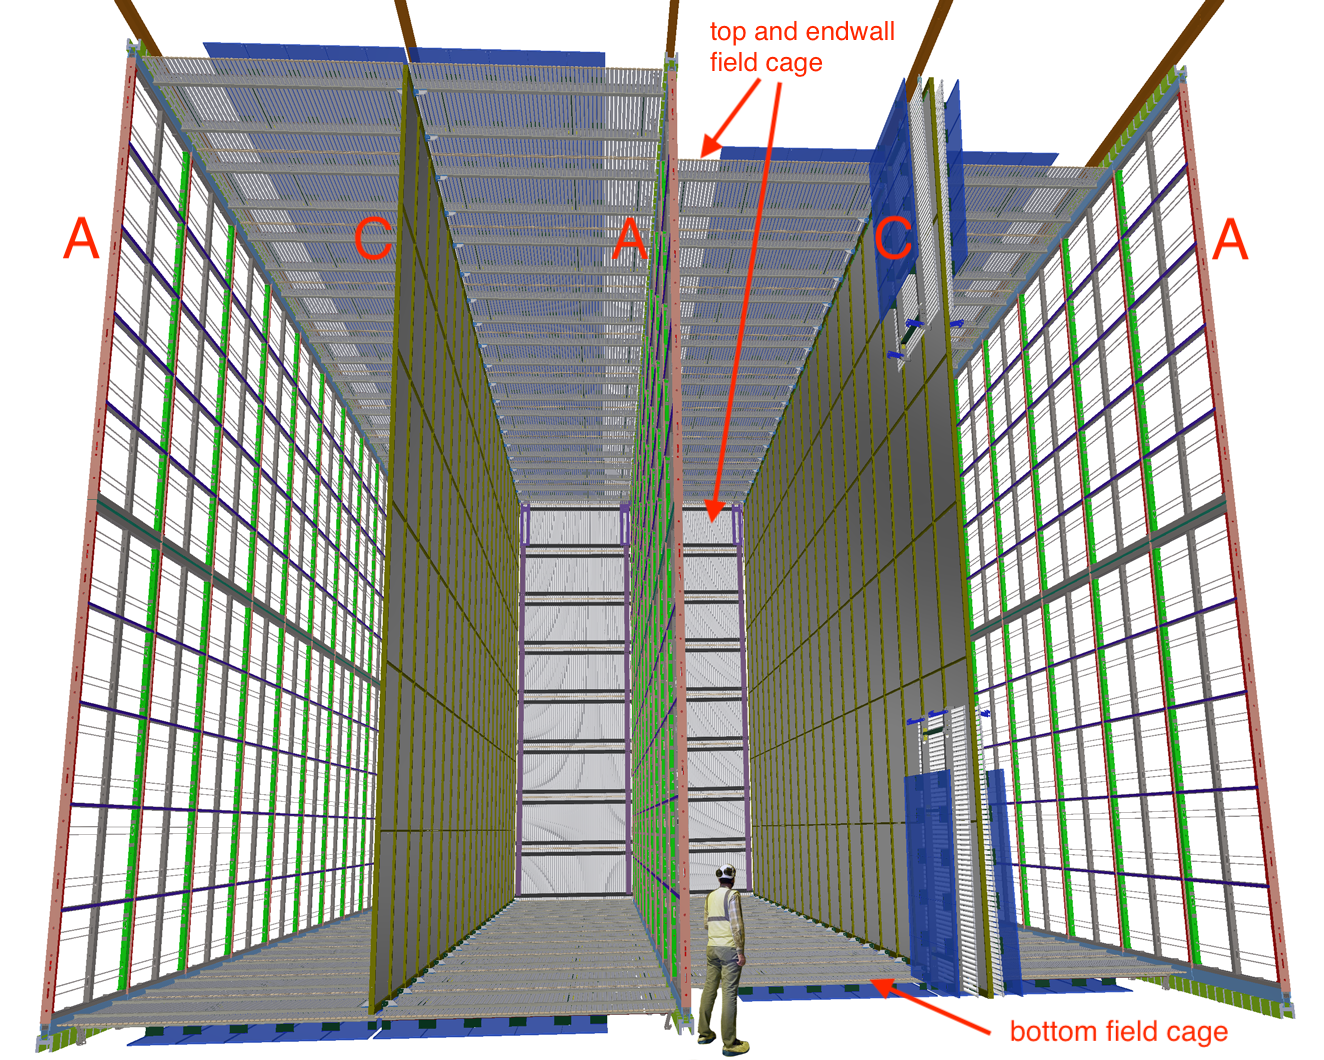
\includegraphics[width=0.8\textwidth]{DUNESchematic.png}
\end{dunefigure}
Figure~\ref{fig:DUNESchematic} 
\end{comment}

Figure~\ref{fig:DUNESchematic1ch1} in Section~\ref{sec:fdsp-exec-splar} shows a \nominalmodsize fiducial mass \dword{spmod} (\larmass total mass); the key parameters of a \dword{spmod} are listed in Table~\ref{tab:sp-key-parameters}. Inside a cryostat of outer dimensions \cryostatlen (L) by \cryostatwdth (W) by \cryostatht{} (H), shown in Figure~\ref{fig:Cryostat}, four \spmaxdrift drift volumes are created between five alternating \dword{apa} and \dword{cpa} arrays, each of dimensions \sptpclen (L) by \tpcheight (H).


\begin{dunetable}
[Key parameters for a \nominalmodsize  \dshort{fd} \dshort{spmod}]
{p{0.65\textwidth}p{0.25\textwidth}}
{tab:sp-key-parameters}
{Key parameters for a \nominalmodsize  \dshort{fd} \dshort{spmod}.}
Item & Quantity   \\ \toprowrule
TPC size & $\tpcheight{}\times\SI{14.0}{\meter}\times\sptpclen{}$ \\ \colhline
Nominal fiducial mass & \spactivelarmass \\ \colhline
\dshort{apa} size & $\SI{6}{\meter}\times\SI{2.3}{\meter}$ \\ \colhline
\dshort{cpa} size & $\SI{1.2}{\meter}\times\SI{4}{\meter}$ \\ \colhline
Number of \dshort{apa}s & 150 \\ \colhline
Number of \dshort{cpa}s & 300 \\ \colhline
Number of \dshort{xarapu} \dshort{pd} bars & 1500 \\ \colhline
\dshort{xarapu} \dshort{pd} bar size & $\SI{209}{\cm}\times\SI{12}{cm}\times\SI{2}{\cm}$ \\ \colhline
Design voltage & \sptargetdriftvolt \\ \colhline
Design drift field & \spmaxfield \\ \colhline
Drift length & \spmaxdrift \\ \colhline
Drift speed & $\SI{1.6}{\mm/\micro\second}$ \\
\end{dunetable}

\begin{dunefigure}[A far detector (\dshort{fd}) cryostat]{fig:Cryostat}{A  \cryostatlen (L) by \cryostatwdth (W) by \cryostatht{} (H) outer-dimension cryostat that houses a \nominalmodsize \dword{fd} module. A mezzanine (light blue) installed \SI{2.3}{m} above the cryostat supports both  detector and cryogenics instrumentation. At lower left, between the \lar recirculation pumps (green) installed on the cavern floor,  the figure of a person indicates the scale.}
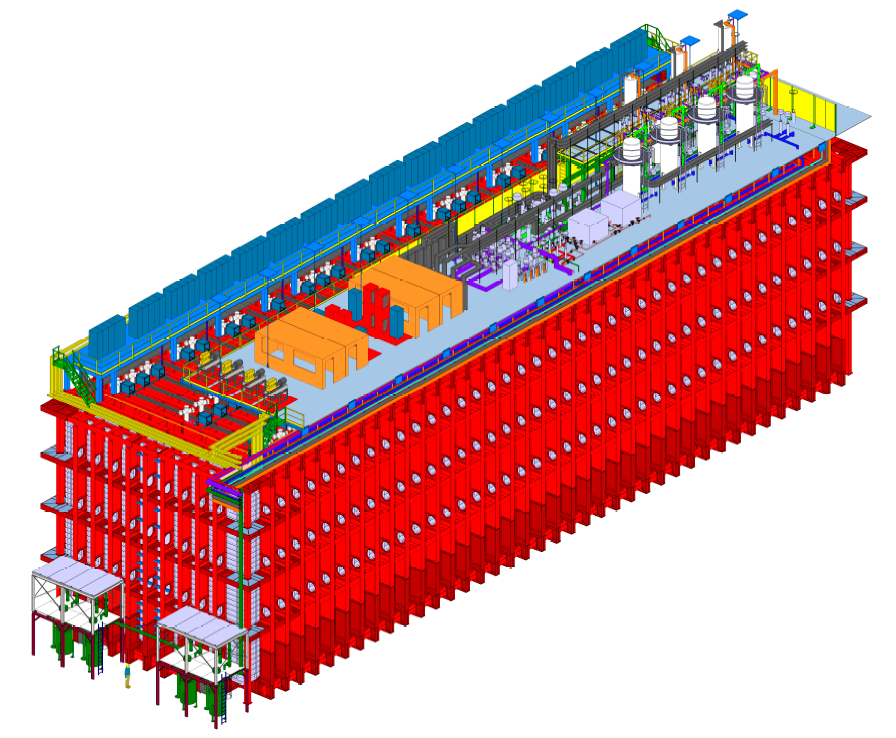
\includegraphics[width=0.8\textwidth]{cryostat-scale.png}
\end{dunefigure}

The target purity from electronegative contaminants in the argon is $<\!100$ \dword{ppt} O$_{2}$ equivalent, enough to ensure a $>\!\SI{3}{\milli\second}$ ionization-electron lifetime at the nominal \SI{500}{\volt/\centi\meter} drift voltage. This target electron lifetime ensures \dword{s/n} of $>\!5$ for the induction planes and $>\!10$ for the collection planes, which are necessary to perform pattern recognition and two-track separation. 

Nitrogen contamination must be $<\!25$ \dword{ppm} to ensure we achieve our requirement of at least 0.5 \phel{}s per MeV detected for events in all parts of the detector, which in turn ensures 
that we can fiducialize nucleon decay events throughout the detector.

\section{Anode Planes}
\label{sec:exec-sp-apa}

The modular anode walls are each made up of 50 \dword{apa}s (25 along the module length and two high), each $\SI{6}{\meter}\times\SI{2.3}{\meter}$. Figure~\ref{fig:APA} shows a schematic and a photograph. As Figure~\ref{fig:APAStack} shows, the \dword{apa}s hang vertically. The \dword{apa}s are two-sided, with three active wire layers and an additional shielding layer, sometimes called a grid layer, wrapped around them. The wire spacing on the layers is $\sim\!\SI{5}{\mm}$. The collection layer is called the $X$ layer; the induction layer immediately next to that is called the $V$ layer; the next induction layer is the $U$ layer; and the shielding layer is the $G$ layer. The $X$ and $G$ layer wires run vertically when installed  (Figure~\ref{fig:APA} shows them horizontal); the $U$ and $V$ layer wires are at $\pm\,\SI{35.7}{\degree}$ to the vertical. The 
wire spacing on each plane defines the spatial resolution of the \dword{apa}; it is wide enough to keep readout costs low and \dword{s/n} high, but small enough to enable reconstruction of 
short tracks such as few-\si{\cm} kaon tracks from proton decay events.

\begin{dunefigure}[An anode plane assembly (APA)]{fig:APA}
{Top: a schematic of an \dword{apa}. The steel \dword{apa} frame is shown in black. The green and magenta lines indicate the directions of the induction wire layers. The blue lines indicate the directions of the induction and shielding (grid) wire layers. The blue boxes at the right end  are the \dword{ce}. Bottom: a \dword{pdsp} \dword{apa} in a wire-winding machine. The end on the right is the head end, onto which the \dword{ce} are mounted.}
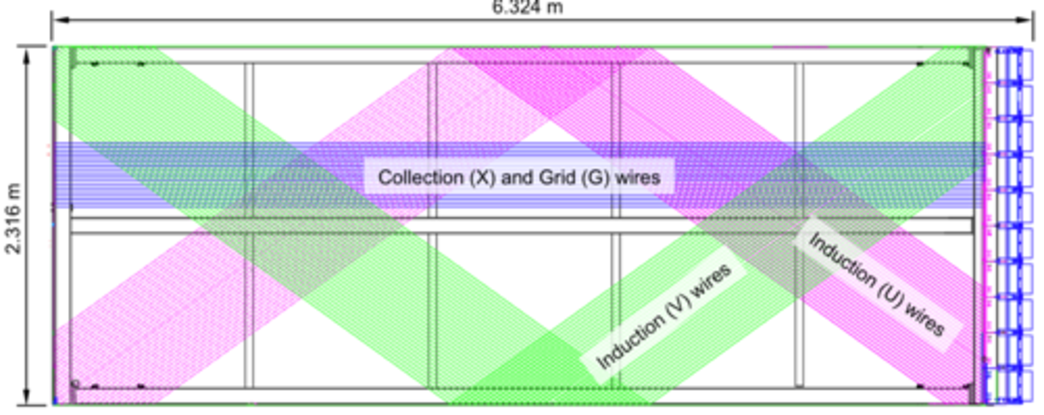
\includegraphics[width=0.7\textwidth]{APASchematic.pdf}
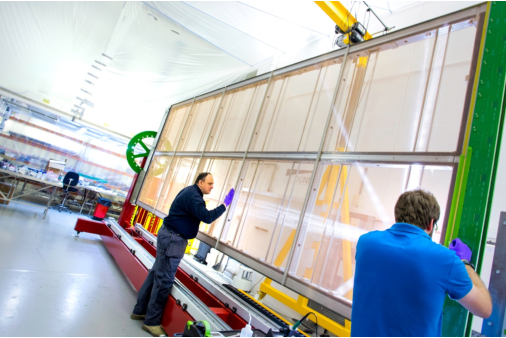
\includegraphics[width=0.6\textwidth]{RealAPA.pdf}
\end{dunefigure}

\begin{dunefigure}[A stack of two APAs]{fig:APAStack}
{Left: two vertically linked \dword{apa}s form one unit of an \dword{apa} array. \dword{pd} bars are installed across the width of the \dword{apa}s. Right: a zoom into only the top and bottom ends of the \dword{apa} stack (notice the breaks in white). This shows the readout electronics and the center of the stack where the \dword{apa}s are connected.}
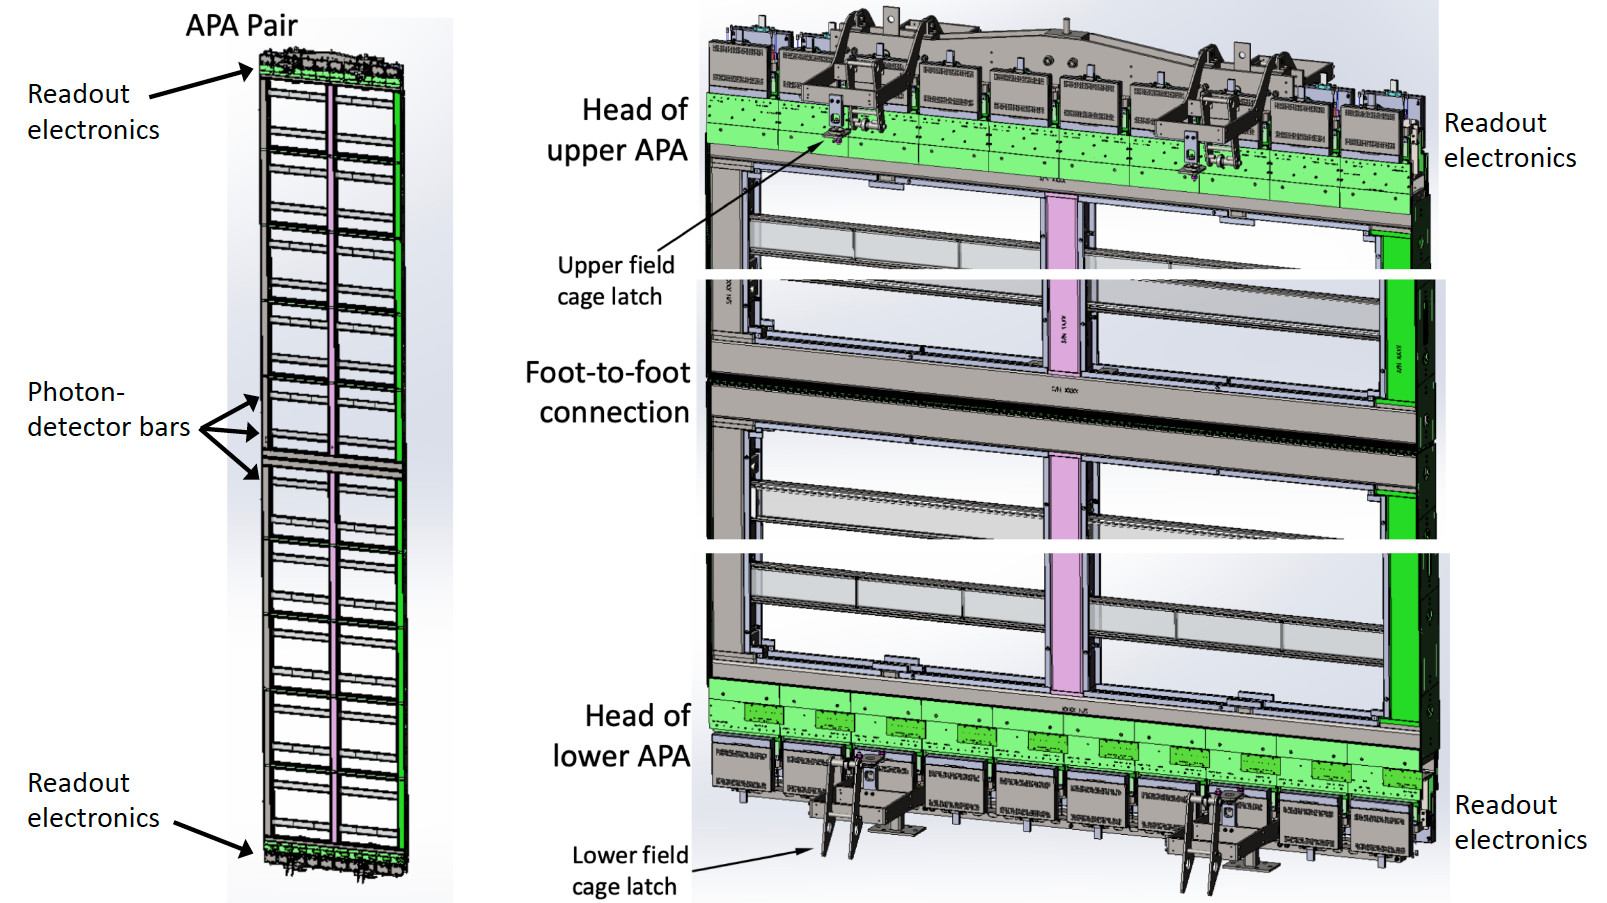
\includegraphics[width=\textwidth]{graphics/APAStack.png}
\end{dunefigure}

\section{Cathode Planes and High Voltage}

Each of the module's two \dfirst{cpa} arrays is formed from 150 \dword{cpa}s (50 along the length, stacked three high), each of which is a $\SI{1.2}{\meter}\times\SI{4}{\meter}$ resistive panel. Each \dword{cpa} has its own independent \dword{hv} supply, providing a current of \SI{0.16}{\milli\ampere} at \sptargetdriftvolt{}. 
With the  \dword{apa} arrays held close to ground, this results in a uniform \spmaxfield \efield across the drift volume.  A typical \dword{mip} passing through the argon produces roughly 60k ionization electrons per centimeter that drift toward the anodes at approximately $\SI{1.6}{\mm/\micro\second}$. The time to cover the full drift distance is about $\SI{2.2}{\milli\second}$.

A \dword{fc} built from field-shaping aluminum profiles surrounds the drift volumes, keeping  the \efield uniform throughout the active \dword{tpc} volume to within 1\%.  The aluminum profiles are connected via a resistive divider chain; between each profile, two \SI{5}{\giga\ohm} resistors, arranged in parallel, provide  \SI{2.5}{\giga\ohm} resistance to create a nominal \SI{3}{\kilo\volt} drop. The \dword{fc} is illustrated in Figure~\ref{fig:FieldCage}.

\begin{dunefigure}[A section of the field cage (FC)]{fig:FieldCage}
{A section of the field cage, showing the extruded aluminum field-shaping profiles, with white polyethylene caps on the ends to prevent discharges.}
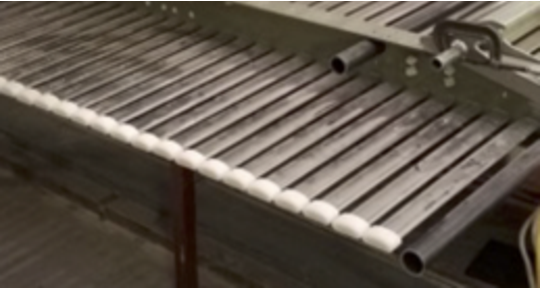
\includegraphics[width=0.5\textwidth]{FieldCage.pdf}
\end{dunefigure}

\section{Electronics}
\label{sec:exec-sp-electronics}

\Dword{fe} readout electronics (in the \dword{lar}), called \dfirst{ce}, are attached to the top end of the top \dword{apa} and the bottom end of the bottom \dword{apa}. 
%These \dword{fe} electronics benefit from the low \dword{lar} temperature because of the reduction in thermal noise. 
Benefitting from a reduction in thermal noise due to the low temperature, the \dword{ce}  
%The \dword{fe} electronics 
shape, amplify, and digitize the signals from the \dword{apa} induction and collection wires thanks to a series of three different types of \dwords{asic} through which all signals pass. 
Outside the cryostat, signals are passed to \dwords{wib} that put the signals onto \SI{10}{\giga\byte} optical fibers, ten per \dword{apa}, which will carry the signals to the upstream \dword{daq} system in the \dword{cuc}. Each \dword{detmodule} has an independent \dword{daq} system that allows it to run as an independent detector, thereby minimizing any chance of a complete \dword{fd} outage. Modules can, however, provide the others with an \dword{snb} trigger signal. The \dword{daq} system also provides the detector clock. 

To enable observation of low-energy particles, we plan to keep noise below $1000\,e^{-}$ per channel, which should be compared to the 20k -- 30k $e^{-}$ per channel collected from a \dword{mip} traveling parallel to the wire plane and perpendicular to the wire orientation. For large signals, we require a linear response up to 500k $e^{-}$, which ensures that fewer than 10\% of beam events experience saturation. This can be achieved using 12\, \dword{adc} bits. %In addition, t
The \dword{ce} are designed with an \dword{fe} peaking time of \SI{1}{\micro\second}, which matches the time for the electrons to drift between wire planes on the \dword{apa}; this leads to a design sampling frequency of \SI{2}{\mega\hertz} to satisfy the Nyquist criterion.

%%%%%%%%%%%%%%%%%%%%%%%%%%%%
\section{Photon Detection System}
\label{sec:fdsp-exec-pds}

In addition to the ionization, charged particles passing through the argon produce approximately 24,000 scintillation photons per \si{\mega\electronvolt}. The scintillation photons are fast, arriving at the \dfirsts{pd} nanoseconds after production. This scintillation light provides a $t_{0}$ for each event. Comparison of the arrival time of ionization at the anode with this $t_{0}$ enables reconstruction in the drift direction. 
The \dword{spmod} implementation enables $\sim\!\SI{1}{\mm}$ position resolution for \SI{10}{\mega\electronvolt} \dword{snb} events. The \dword{pd} $t_{0}$ is also vital in fiducializing nucleon decay events, which allows us to reject cosmic-muon-induced background events that will occur near the edges of the detector modules.

The photons are collected by devices called \dwords{xarapu}, which are mounted in the \dword{apa} frames between the sets of wire layers, as shown in Figure~\ref{fig:APAStack}. 
The \dwords{xarapu} %bars 
consist of layers of dichroic filter and wavelength-shifter, illustrated in Figure~\ref{fig:ArapucaCell}, that shift the \dword{vuv} scintillation light into the visible range  trap  the visible photons, %transporting 
and transport them to \dword{sipm} devices. The signals from these \dwords{sipm} are sent along cables that pass through the hollow \dword{apa} frames, up to feedthroughs in the cryostat roof. The \dword{pd} and \dword{apa}-wire data-streams are merged at the \dword{daq}. 

\dword{pd} modules, shown in Figure~\ref{fig:PDModules}, are 
$\SI{209}{\cm}\times\SI{12}{\cm}\times\SI{2}{\cm}$ bars that each hold 24 \dwords{xarapu}. 
Ten \dword{pd}  modules  are mounted in each \dword{apa} between the wire layers. 

\begin{dunefigure}[An \dshort{xarapu} photon detector (PD) cell]{fig:ArapucaCell}
{Left: an \dword{xarapu} cell. Right: an exploded view of the \dword{xarapu} cell, where the blue sheet is the \dword{wls} plate and the yellow sheets are the dichroic filters.}
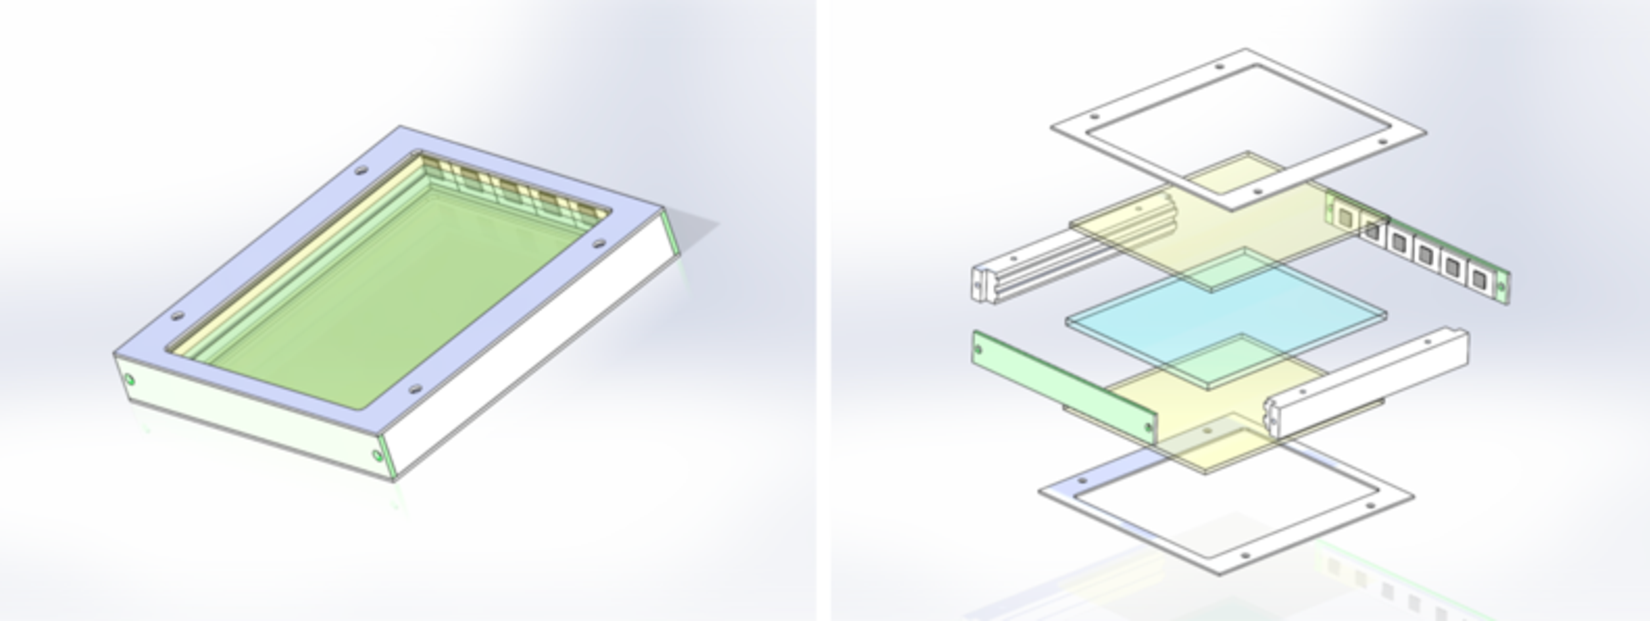
\includegraphics[width=\textwidth]{XArapuca.pdf}
\end{dunefigure}

\begin{dunefigure}[PD modules mounted in an APA]{fig:PDModules}
{Left: an \dword{xarapu} \dword{pd} module. The 48 \dwords{sipm} that detect the light from the 24 cells are along the long edges of the module. Right: \dword{xarapu} \dword{pd} modules mounted inside an \dword{apa}.}
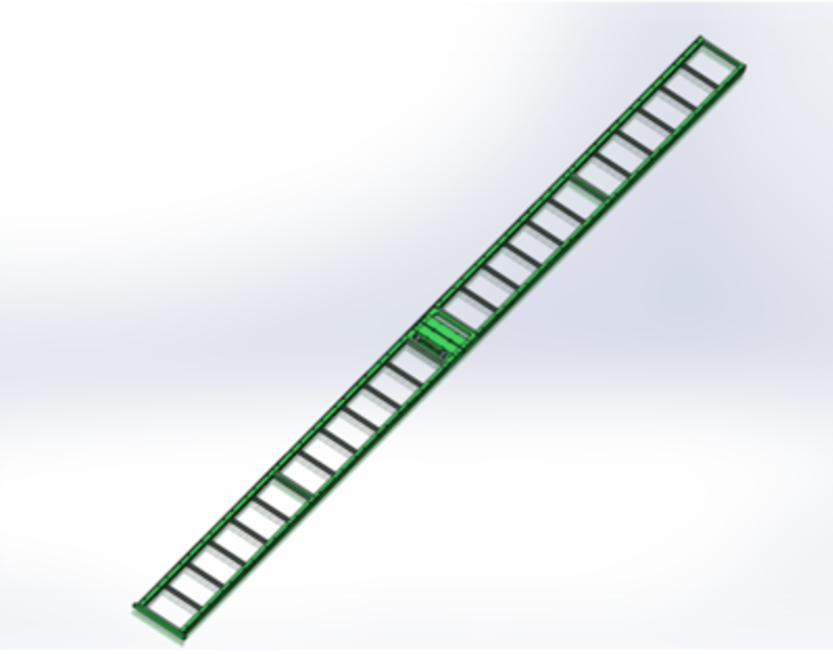
\includegraphics[width=0.49\textwidth]{PDBar.pdf}
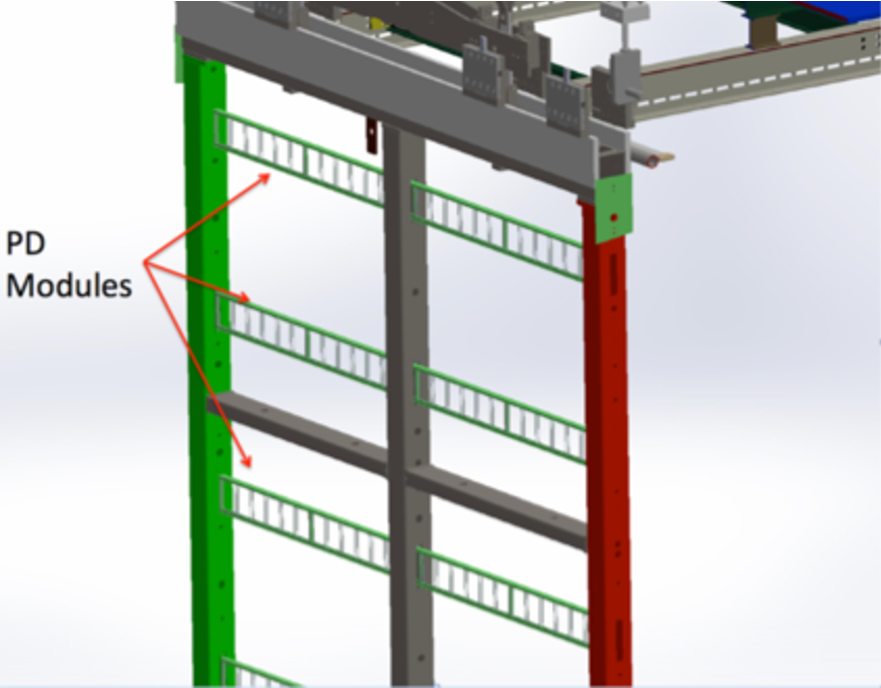
\includegraphics[width=0.49\textwidth]{PDsInAPA.pdf}
\end{dunefigure}


The 48 \dword{sipm}s on each \dword{xarapu} supercell are ganged together, and the signals are collected by \dword{fe} electronics, mounted on the supercell. The design of the \dword{fe}  electronics is inspired by the system used for the \dword{mu2e} cosmic-ray tagger~\cite{bib:mu2e_tdr}, which uses commercial ultrasound \dwords{asic}. The \dword{fe} electronics define the \SI{1}{\micro\second} timing resolution of the \dword{pd} system.

%%%%%%%%%%%%%%%%%%%%%%%%%%%
\section{Calibration}
\label{sec:exec-sp-calibration}

The challenge of calibrating the \dword{dune} \dword{fd} is controlling the response of a huge cryogenic detector over a period of decades, a challenge amplified by the detector's location deep underground and therefore shielded from the cosmic muons that have typically been used as standard candles for %previous 
\dwords{lartpc}.  The \dword{fd} calibration system  has been designed jointly for the \dword{sp} and \dword{dp} technologies, and uses the same strategies and systems for both.

To achieve our \si{\giga\electronvolt}-scale oscillation and nucleon decay physics goals, we must know our fiducial volume to 1 -- 2\% and have a similar understanding of the vertex position resolution; understand the \nue event rate to 2\%; and control our lepton energy scales to 1\% and hadron energy scales to 3\%. At the \si{\mega\electronvolt} scale, our physics requirements are driven by our goal of identifying and measuring the spectral structure of an \dword{snb}; here, we must achieve a 20 -- 30\% energy resolution, understand our event timing to the \SI{1}{\micro\second} level, and measure our trigger efficiency and levels of radiological background. 

The tools available to us for calibration include the \dword{lbnf} beam, atmospheric neutrinos, atmospheric muons, radiological backgrounds, and dedicated calibration devices installed in the detector. At the lowest energies, we have deployable neutron sources and intrinsic radioactive sources; in particular, the natural $^{39}$Ar component of the \dword{lar} with its \SI{565}{\kilo\electronvolt} end-point, given its pervasive nature across the detector, can be used to measure the spatial and temporal variations in electron lifetime. The possibility of deploying radioactive sources is also under study. %being explored. 
In the \SIrange{10}{100}{\mega\electronvolt} energy range, we will use Michel electrons, photons from $\pi^{0}$ decay, stopping protons, and both stopping and through-going muons. We will also have built-in lasers, purity monitors, and thermometers, as well as the ability to inject charge into the readout electronics. Finally, data from the \dword{protodune} detectors  (Section~\ref{sec:exec:overall:pdune}) will be invaluable in understanding the response and \dword{pid} capabilities of the \dword{fd}.

Over time, the \dword{fd} calibration program will evolve as statistics from cosmic rays and the \dword{lbnf} beam amass and add to the information gained from the calibration hardware systems. These many calibration tools will work alongside the detector monitoring system, the \dword{cfd} models of the argon flow, and \dword{protodune} data to give us a detailed understanding of the \dword{fd} response across the \dword{dune} physics program.

%%%%%%%%%%%%%%%%%%%%%%%%%%%%%%%%%%%
\section{Data Acquisition}
\label{sec:exec-sp-daq}

The \dword{daq} systems for the \dword{sp} and \dword{dp} technologies have been designed jointly and are identical except for the architecture of the detector readout electronics.  
The output format of the generated data is common, and both are synchronized to the same global clock signals.  The \dword{daq} architecture is based on the \dword{felix} system designed at \dshort{cern} and used for the \dword{lhc} experiments. 

The \dword{daq} is divided between an upstream section, located underground in the \dword{cuc}, and a downstream \dword{daqbes} to be located above ground at the \dword{surf}. All trigger decisions are made 
upstream, and the data is buffered underground until the \dword{daqbes} indicates it is ready to receive data; this controls the rate of data flowing to the surface. An end-goal of the \dword{daq} is to achieve a data rate to tape of no more than \SI{30}{\peta\byte/\year}.

For the \dword{spmod}, the 150 \dword{apa}s are processed by 75 \dwords{daqrou}; each \dword{daqrou} contains one \dword{felix} board. The \dwords{pd} from the module will have a lower data rate because the \dword{pd} electronics, unlike the \dword{tpc} electronics, perform zero-suppression; therefore, the \dwords{pd} of a module will be processed by six to eight additional \dwords{daqrou}. The \dword{daq} can be partitioned: it will be possible to run multiple instances of the \dword{daq} simultaneously, so most of the detector can be taking physics data while other \dword{daq} instances are doing test runs for development or special runs such as calibration runs. 

Two basic triggers will be operating. Beam, cosmic, and nucleon decay events will be triggered using the localized high-energy trigger 
that will open a readout window of \SI{5.4}{\ms}, enough to read out the full \dword{tpc} drift around an event. For \dwords{snb}, we will use an extended low-energy trigger. This will look for coincident regions of low-energy deposits, below \SI{10}{\mega\electronvolt}, across an entire module and in a \SI{10}{\second} period. An extended high-energy trigger will open a readout window of \SI{100}{\second} to capture a full \dword{snb}. 

The \dword{daq} must also provide the system clock that keeps the detector components synchronized and %provides the timestamp for 
timestamps all data. The timestamp derives from a \dword{gps} \dword{pps} fed into the \dword{daq} with \SI{1}{\micro\second} precision, adequate %to timestamp 
for beam and \dword{snb} events. To provide finer synchronization between detector components, a \SI{10}{\mega\hertz} reference clock drives the module's \SI{62.5}{\mega\hertz} master clock, which is fanned out to all detector components, providing an overall synchronization to a precision of \SI{1}{\nano\second}.



%%%%%%%%%%%%%%%%%%%%%%%%%%%%%%%%%%%
\section{Cryogenics Instrumentation and Slow Controls}
\label{sec:dp-execsum-sc}

\fixme{Anne rewrote this from text from the SP/DP volumes because the previous text was DP-centric. Somebody should check this.}

\dword{dune}'s \dword{cisc} system is responsible for recognizing and preventing fault conditions that could develop in a \dword{detmodule} over long periods of running. 
The \dword{sp} and \dwords{dpmod} will use a \dword{cisc} system that has been designed jointly.

Cryogenics instrumentation includes purity monitors,  various types of temperature monitors, and cameras with their associated light emitting systems. Also included are %components like 
gas analyzers and \dword{lar} level monitors that are directly related to the external cryogenics system, which have substantial interfaces with \dword{lbnf}. %\dword{lbnf} provides the needed expertise  for these systems and is responsible for the design, installation, and commissioning, while the \dword{cisc} consortium provides the resources and supplements labor as needed. 

Cryogenics instrumentation %also 
requires significant engineering, physics, and
simulation work, such as \efield simulations and cryogenics modeling
studies using \dfirst{cfd}. \efield simulations
%are required to 
identify desirable locations for instrumentation
devices in the cryostat, away from %so they are not in 
regions of high \efield, so that %and 
their presence does not induce large field distortions. 
\dword{cfd} simulations help identify %are needed to understand 
expected temperature, impurity, and velocity flow distributions and guide the placement and distribution of instrumentation devices inside the cryostat.

The slow controls portion of \dword{cisc} consists of three main components: 
hardware, infrastructure, and software. The slow controls hardware and infrastructure comprises networking hardware, signal processing hardware, computing hardware, and associated rack infrastructure. The slow controls software provides, for every slow control quantity, the central slow controls processing architecture, databases, alarms, archiving, and control room displays.


%%%%%%%%%%%%%%%%%%%%%%%%%%%%%%%%%%%
\section{Installation}

A significant challenge for \dword{dune} is transporting all detector and infrastructure components down the \SI{1500}{\meter} Ross shaft and through drifts to a detector cavern. The 150 \dwords{apa}, each \SI{6.0}{m} high and \SI{2.3}{m} wide, and  weighing \SI{600}{kg} with $3500$ strung sense and shielding wires, must be taken down the shaft as special ``slung loads,'' presenting an extra challenge. 

Once the \dword{spmod} cryostat is ready, %has been installed, 
a \dword{tco} is left open at one end through which the detector components are installed. A cleanroom is built around the \dword{tco} to prevent any contamination entering the cryostat during installation. The \dword{dss} is then installed into the cryostat, ready to receive the \dword{tpc} components. 

In the cleanroom the \dword{apa}s are outfitted  with \dword{pd} units and passed through a series of qualification tests.
Two \dword{apa}s are linked into a vertical \SI{12}{m} high double unit and connected to readout electronics. 
They are tested in a \coldbox, then move into the cryostat to be installed at the proper location on the \dword{dss}, and have their cabling connected to \fdth{}s. 
The \dword{fc}, \dwords{cpa} and their \dword{hv} connections, elements of the \dword{cisc}, and detector calibration systems are installed in parallel with the \dword{apa}s. 

After twelve months of detector component installation, the \dword{tco} closes (the last installation steps occur in a confined space accessed through a narrow human-access port on top of the cryostat). 
Following leak checks, final electrical connection tests, and installation of the neutron calibration source, the process of filling the cryostat with \SI{17000000}{\kilo\gram} of \dword{lar} begins.

To help plan the installation phase, installation tests will be performed at the \dword{nova} \dword{fd} site in \dword{ashriver}, Minnesota, USA. These tests will allow us to develop our procedures, train installation workers, and develop our labor planning through time and motion studies. Throughout the project, safety, \dword{qa}, and \dword{qc} are written into all processes.

Safety of both personnel and  detector components is the paramount consideration throughout the installation process and beyond. Once the detectors are taking data, %safety is still the priority with 
the \dword{ddss} will be monitoring for argon level drops, water leaks, and smoke. A detailed detector and cavern grounding scheme has been developed that not only guards against ground loops but also ensures that any power faults are safely shunted to the facility ground.

